\chapter{Modelli} \label{ch:modelli}
In questo capitolo verranno presentati i modelli che sono stati definiti
per svolgere il compito di classificazione. In particolare, si è deciso di
utilizzare i seguenti algoritmi:
\begin{itemize}
    \item \textbf{Support Vector Machine}
    \item \textbf{Gaussian Naive Bayes}
    \item \textbf{Rete Neurale}
\end{itemize}
Per ogni algoritmo sono stati definiti $2$ modelli, ciascuno allenato e valutato
sulle due versioni ridotte del dataset originario. Nella tabella
\ref{tab:riassunto_operazioni_dataset} viene mostrato un breve riepilogo delle
versioni dei dataset e dei modelli che verranno definiti.

\begin{table}[!ht]
    \resizebox{\textwidth}{!}{\begin{tabular}{@{}llc@{}}
            \toprule
            \rowcolor[HTML]{EFEFEF}
            \textbf{Nome del dataset}                                                                                          &
            \textbf{Operazioni applicate}                                                                                      &
            \multicolumn{1}{l}{\cellcolor[HTML]{EFEFEF}\textbf{Utilizzato per i seguenti modelli}}                                                                                                      \\ \midrule
            \texttt{dataset\_corr}                                                                                             &
            \begin{tabular}[c]{@{}l@{}}Riduzione della dimensionalità utilizzando l'analisi \\ della correlazione\end{tabular} &
            GNB\_corr                                                                                                                                                                                   \\
            \texttt{dateset\_corr\_std}                                                                                        & dataset\_corr con la standardizzazione dei dati & SVM\_corr e NN\_corr \\
            \texttt{dateset\_pca}                                                                                              & dataset\_corr\_std applicando l'algoritmo PCA   & GNB\_pca             \\
            \texttt{dateset\_pca\_std}                                                                                         & dataset\_pca con la standardizzazione dei dati  & SVM\_pca e NN\_pca   \\ \bottomrule
        \end{tabular}}
    \caption{Riassunto delle operazioni effettuate sui dataset e utilizzo dei dataset per i modelli.}
    \label{tab:riassunto_operazioni_dataset}
\end{table}

Successivamente, per ogni versione di ciascun modello saranno presentate due
tipologie di valutazione delle performance:
\begin{itemize}
    \item \textbf{Valutazione $80/20$}: si effettuano gli apprendimenti di
          ciascuna versione sull'$80\%$ del dataset di riferimento e si testa
          la versione del modello sul $20\%$ del dataset di riferimento rimanente.
    \item \textbf{Cross-validation}: si effettua una $10$-fold stratified
          cross-validation per studiare la robustezza della versione del modello
          testata precedentemente.
\end{itemize}


La scelta di effettuare una valutazione in due fasi si basa sul fatto che il
numero degli esempi presenti nel dataset non è molto elevato, più precisamente
il dataset è di medie dimensioni, quindi la valutazione $80/20$ potrebbe non
essere sufficiente. La seconda valutazione si effettua per verificare la
robustezza dei modelli creati, calcolando gli intervalli di confidenza delle
metriche di valutazione.

La porzione di dati dedicata all'addestramento dei modelli, composta dall'$80\%$
delle istanze, è anche stata utilizzata anche per ricercare gli iperparamentri
migliori per la rete neurale e per la SVM tramite l'utilizzo di una $5$-fold 
stratified cross-validation.
\section{Support Vector Machine}
In questa sezione verrà presentato il processo di addestramento e selezione dei
modelli candidati per \textbf{SVM}. Nello specifico si andranno a presentare le
varie scelte effettuate per la definizione di ciascun modello tramite la selezione
degli iperparametri e la valutazione dei risultati ottenuti durante il loro studio.
Tutte le operazioni effettuate sono state realizzate utilizzando i dataset standardizzati
(\texttt{dataset\_corr\_std} e \texttt{dataset\_pca\_std}) presentati nella fase
di preparazione dei dati, in modo da rispettare il più possibile le assunzioni
di SVM, anche se una feature non rispetta l'ipotesi di normalità.

In questa sezione verranno presentati i seguenti modelli:
\begin{itemize}
    \item SVM\_corr: utilizza SVM su \texttt{dataset\_corr\_std}
    \item SVM\_pca: utilizza SVM su \texttt{dataset\_pca\_std}
\end{itemize}

\subsection{Modello SVM\_corr}
La prima fase di definizione del modello, si è delineata nella selezione degli
iperparamentri migliori per il classificatore SVM, la quale è stata
condotta mediante l'impiego di procedure di grid search. Nello specifico, si è
adottata una grid search per ciascun kernel, utilizzando una tecnica di
cross-validation a $5$ fold. Tale decisione risulta necessaria data la presenza
di iperparametri specifici per ciascun kernel. Considerando che i
kernel presentano parametri differenti da ottimizzare, il processo di selezione
deve affrontare un elevato numero di combinazioni, il che potrebbe generare
combinazioni prive di significato se svolto in un unico processo. Pertanto, sono
stati valutati i seguenti kernel:
\begin{itemize}
    \item Lineare.
    \item Polinomiale.
    \item RBF.
    \item Sigmoidale.
\end{itemize}

Per effettuare il processo di selezione degli iperparametri, si è deciso di
effettuare uno studio preliminare per valutare quali fossero quelli più
significativi per ogni kernel, in modo da non doverli analizzare tutti e di
conseguenza ridurre il tempo di esecuzione. Lo studio si è basato sull'esecuzione
dell'algoritmo SVM, facendo variare manualmente tutti gli iperparametri, in questo
modo si è notato che i parametri che facevano variare maggiormente i risultati
dei modelli erano i seguenti:
\begin{itemize}
    \item \textbf{Parametro di regolarizzazione} ($C$): controlla il trade-off tra
          la complessità del modello e la corretta classificazione dei dati.
          Un suo valore elevato porta ad avere un hard margin.
    \item \textbf{Tolleranza} ($tol$): parametro di tolleranza, controlla la
          tolleranza accettata per la convergenza del modello.
    \item \textbf{Coefficiente di bias} ($r$): termine indipendente di bias che
          controlla la posizione dell'iperpiano di separazione nel caso di
          kernel polinomiale e sigmoidale.
    \item \textbf{Grado del polinomio} ($d$): controlla la complessità del modello
          impostando il grado del polinomio. Utile solo per il kernel polinomiale.
    \item \textbf{Coefficiente di scala} ($\boldsymbol{\gamma}$): specifica il learning
          rate per i kernel polinomiali, rbf e sigmoidali.
    \item \textbf{Numero massimo di iterazioni}($max\_iter$): indica il numero massimo
          di iterazioni consentite.
\end{itemize}

Selezionati i parametri più significativi, si è proceduto con la grid search
per trovare le combinazioni migliori per il dataset di riferimento. Per valutare
ogni combinazione di iperparamentri, si calcola la media e la deviazione standard
dell'Accuracy (test score) e del tempo di addestramento per i $5$ modelli della $5$-fold
cross-validation.
In seguito, si è attribuito un punteggio di ranking per ogni combinazione
di iperparamentri in relazione al suo posizionamento rispetto all'Accuracy e rispetto
al tempo. Infine, sommando i due valori di rank, si ottiene il punteggio di ranking
della combinazione.

In questo modo è stata scelta la combinazione migliore per ogni kernel, ovvero quella che possiede la somma
con punteggio di ranking più basso rispetto alle altre combinazioni, in quanto rappresenta
il miglior compromesso tra accuratezza e tempo.

Inoltre si fa presente che per il kernel lineare e polinomiale è stato impostato
un numero massimo di iterazioni pari a $100000$ per rimanere competitivi con i
tempi essendo che alcune combinazioni di iperparametri rallentavano notevolmente
il tempo di convergenza del modello.

\subsubsection{Kernel lineare $\langle x,x'\rangle$}
Il kernel lineare si limita ad effettuare il prodotto scalare tra due vettori,
risultando particolarmente utile quando i dati sono linearmente separabili.
Per questo motivo sono stati valutati solamente i seguenti iperparamentri:
\begin{itemize}
    \item \textbf{Parametro di regolarizzazione} ($C$): valori testati sono stati $1$,
          $100$, $1e6$.
    \item \textbf{Tolleranza} ($tol$): valori testati sono stati $1e-2$, $1e-3$, $1e-5$.
\end{itemize}
Nella tabella \ref{tab:top_linear_corr} viene riportato il miglior candidato per il kernel lineare:
\begin{table}[!ht]
    \centering
    \begin{tabular}{@{}ccccc@{}}
        \toprule
        \rowcolor[HTML]{EFEFEF}
        \textbf{params} & \textbf{mean\_fit\_time} & \textbf{std\_fit\_time} & \textbf{mean\_test\_score} & \textbf{std\_test\_score} \\ \midrule
        C: 1, tol: 0.01 & 0.058                    & 0.015                   & 0.9824                     & 0.0048                    \\ \bottomrule
    \end{tabular}
    \caption{Miglior candidato per il kernel lineare}
    \label{tab:top_linear_corr}
\end{table}
\subsubsection{Kernel polinomiale $(\gamma\langle x,x'\rangle + r)^d$}
Il kernel polinomiale si occupa di trasformare i dati in uno spazio di
feature di dimensione superiore utilizzando la funzione polinomiale.
Solo per questo tipo di kernel è stata presa la decisione di impostare
una tolleranza alta comune a tutte le combinazioni per raggiungere più
velocemente la convergenza. Sono stati ottimizzati i seguenti iperparamentri:
\begin{itemize}
    \item \textbf{Parametro di regolarizzazione} ($C$): valori testati sono stati $1$,
          $100$, $1e3$. Da notare che è stato abbassato il valore massimo di $C$ in
          quanto per valori più elevati il modello non riusciva ad ottenere dei
          risultati validi per il limite massimo di iterazioni.
    \item \textbf{Coefficiente di bias} ($r$): valori testati sono stati $10.0$, $1$, $0.1$.
    \item \textbf{Grado del polinomio} ($d$): valori testati sono stati $2$, $3$, $4$.
    \item \textbf{Coefficiente di scala} ($\boldsymbol{\gamma}$): valori testati sono stati
          $'scale'$, $'auto'$, $1e-3$, $1$, $1e3$.
\end{itemize}

Nella tabella \ref{tab:top_poly_corr} viene riportato il miglior candidato per il kernel polinomiale:
\begin{table}[!ht]
    \centering
    \begin{tabular}{@{}ccccc@{}}
        \toprule
        \rowcolor[HTML]{EFEFEF}
        \textbf{params}                    & \textbf{mean\_fit\_time} & \textbf{std\_fit\_time} & \textbf{mean\_test\_score} & \textbf{std\_test\_score} \\ \midrule
        C: 1, r: 10, d: 3, $\gamma$: scale & 0.075                    & 0.003                   & 0.9895                     & 0.003                     \\ \bottomrule
    \end{tabular}
    \caption{Miglior candidato per il kernel polinomiale}
    \label{tab:top_poly_corr}
\end{table}
\subsubsection{Kernel RBF $\exp(-\gamma|| x-x'||^2)$}
Anche il kernel RBF si occupa di trasformare i dati in uno spazio di
feature di dimensione superiore tramite la funzione esponenziale.
In questo caso non viene più effettuato il prodotto scalare tra i vettori ma si misura
la loro distanza euclidea, questo tende a creare frontiere decisionali radiali.
Per RBF sono stati ottimizzati i seguenti iperparamentri:
\begin{itemize}
    \item \textbf{Parametro di regolarizzazione} ($C$): valori testati sono stati $1$, $100$, $1e6$.
    \item \textbf{Coefficiente di scala} ($\boldsymbol{\gamma}$): valori $'scale'$, $'auto'$, $1e-3$, $1$, $1e3$.
\end{itemize}

Nella tabella \ref{tab:top_rbf_corr} viene riportato il miglior candidato per il kernel rbf:
\begin{table}[!ht]
    \centering
    \begin{tabular}{@{}ccccc@{}}
        \toprule
        \rowcolor[HTML]{EFEFEF}
        \textbf{params}        & \textbf{mean\_fit\_time} & \textbf{std\_fit\_time} & \textbf{mean\_test\_score} & \textbf{std\_test\_score} \\ \midrule
        C: 100, $\gamma$: auto & 0.055                    & 0.002                   & 0.9915                     & 0.0035                    \\ \bottomrule
    \end{tabular}
    \caption{Miglior candidato per il kernel rbf}
    \label{tab:top_rbf_corr}
\end{table}

\subsubsection{Kernel sigmoidale $\tanh(\gamma\langle x,x'\rangle + r)$}
Il kernel sigmoidale si occupa di trasformare i dati in uno spazio di
feature di dimensione superiore tramite la funzione tangente iperbolica
ispirandosi alla funzione di attivazione nelle reti neurali.
Questo kernel è risultato molto sensibile rispetto ai parametri $\gamma$ e $r$, ma
dal momento che non presentava combinazioni con esecuzioni onerose a livello di 
complessità temporale si è deciso di ottimizzare anche quegli iperparametri che
hanno ricoperto un ruolo meno significativo durante la fase preliminare della
grid search.

Sono stati ottimizzati i seguenti iperparamentri:
\begin{itemize}
    \item \textbf{Parametro di regolarizzazione} ($C$): valori testati sono stati $1$, $100$, $1e6$.
    \item \textbf{Coefficiente di bias} ($r$): valori testati sono stati $-1$, $0$, $1$.
    \item \textbf{Tolleranza} ($tol$): valori testati sono stati $1e-2$, $1e-3$, $1e-5$.
    \item \textbf{Coefficiente di scala} ($\boldsymbol{\gamma}$): valori testati sono stati $'scale'$ e $'auto'$.
\end{itemize}

Nella tabella \ref{tab:top_sigmoid_corr} viene riportato il miglior candidato per il kernel sigmoidale:
\begin{table}[!ht]
    \centering
    \begin{tabular}{@{}ccccc@{}}
        \toprule
        \rowcolor[HTML]{EFEFEF}
        \textbf{params}                          & \textbf{mean\_fit\_time} & \textbf{std\_fit\_time} & \textbf{mean\_test\_score} & \textbf{std\_test\_score} \\ \midrule
        C: 1, r: 0.0, $\gamma$: scale, tol: 0.01 & 0.071                    & 0.003                   & 0.9077                     & 0.0112                    \\ \bottomrule
    \end{tabular}
    \caption{Miglior candidato per il kernel sigmoidale}
    \label{tab:top_sigmoid_corr}
\end{table}

\subsubsection{Selezione miglior kernel}
La fase successiva è stata quella di confrontare le combinazioni migliori per ogni
kernel per determinare la migliore per il dataset. I risultati a livello di tempi sono
riportati nella tabella \ref{tab:top_time_kernels_corr}.
\begin{table}[!ht]
    \centering
    \begin{tabular}{@{}lcc@{}}
        \toprule
        \rowcolor[HTML]{EFEFEF}
        \multicolumn{1}{c}{\cellcolor[HTML]{EFEFEF}\textbf{kernel}} & \textbf{mean\_fit\_time} & \textbf{std\_fit\_time} \\ \midrule
        Linear                                                      & 0.058                    & 0.015                   \\
        Poly                                                        & 0.075                    & 0.003                   \\
        Rbf                                                         & 0.055                    & 0.002                   \\
        Sigmoid                                                     & 0.071                    & 0.003                   \\ \bottomrule
    \end{tabular}
    \caption{Risultati dei tempi delle migliori combinazioni per kernel}
    \label{tab:top_time_kernels_corr}
\end{table}

Successivamente per ogni kernel riaddestrato sono state calcolate
le metriche, ossia:
\begin{itemize}
    \item Accuratezza
    \item Precision
    \item Recall
    \item F1-score
\end{itemize}
e le relative curve ROC.

\begin{table}[!ht]
    \centering
    \begin{tabular}{@{}lcccc@{}}
        \toprule
        \rowcolor[HTML]{EFEFEF}
        \multicolumn{1}{c}{\cellcolor[HTML]{EFEFEF}\textbf{kernel}} & \textbf{Accuracy} & \textbf{Precision} & \textbf{Recall} & \textbf{F1-score} \\ \midrule
        Linear                                                      & 97.97\%           & 99.69\%            & 95.81\%         & 97.71\%           \\
        Poly                                                        & 98.51\%           & 99.39\%            & 97.31\%         & 98.34\%           \\
        Rbf                                                         & 98.11\%           & 99.38\%            & 96.41\%         & 97.87\%           \\
        Sigmoid                                                     & 88.78\%           & 87.24\%            & 88.02\%         & 87.63\%           \\ \bottomrule
    \end{tabular}
    \caption{Risultati delle metriche principali per kernel}
    \label{tab:top_metrics_kernels_corr}
\end{table}
\begin{figure}[!ht]
    \centering
    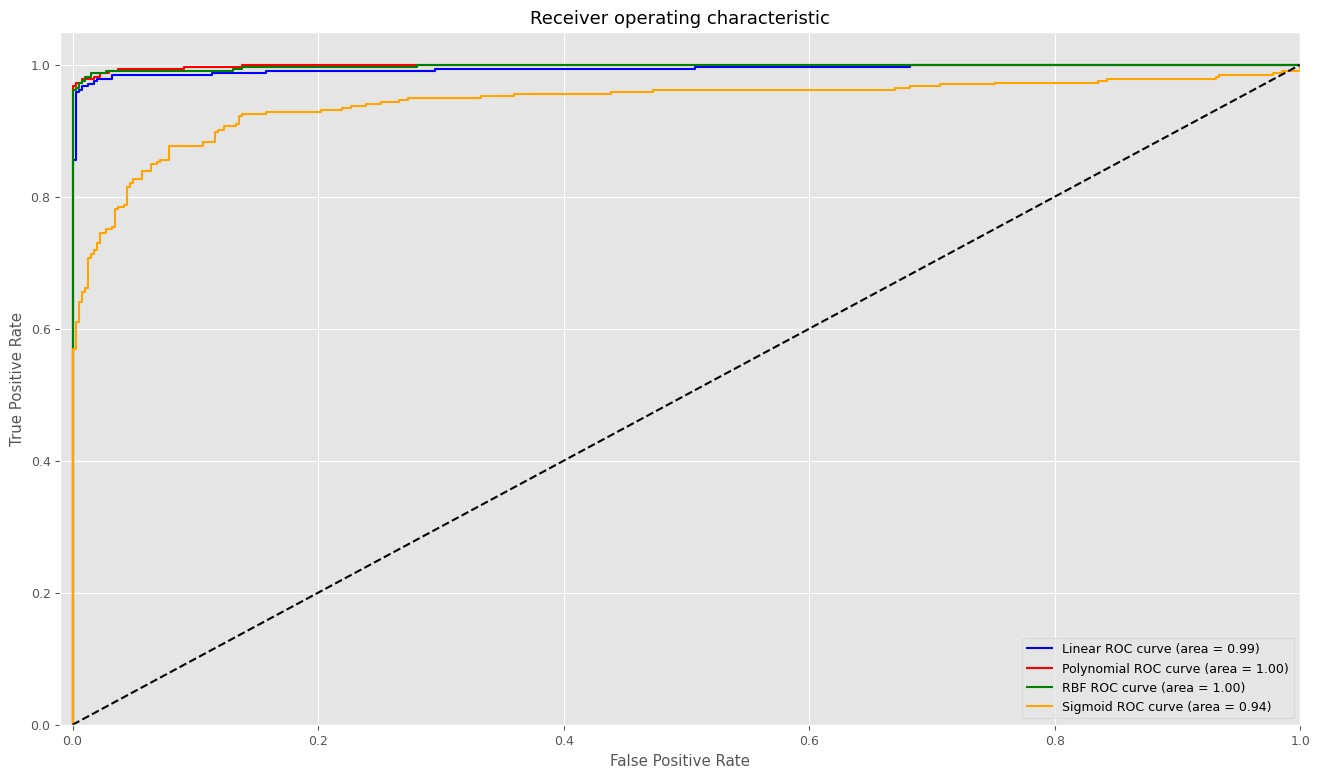
\includegraphics[width=0.75\textwidth]{img/svm/roc_SVM.png}
    \caption{Curva ROC dei vari kernel SVM a confronto}
    \label{fig:roc_SVM_corr}
\end{figure}

Dalla tabella \ref{tab:top_metrics_kernels_corr} si può notare che il kernel Polinomiale
è quello che ha ottenuto i risultati migliori, quindi il modello SVM\_corr sarà
definito dai seguenti parametri:
\begin{itemize}
    \item kernel: $polinomiale$
    \item $C$: $1$
    \item $r$: $10$
    \item $d$: $3$
    \item $\gamma$: $scale$
\end{itemize}

Bisogna notare però che dal confronto delle curve roc \ref{fig:roc_SVM_corr} e
dalle metriche i risultati ottenuti sono ottimi per tutti
i kernel escludendo la sigmoide.

\subsection{Modello SVM\_pca}
La prima fase di definizione del modello, si è delineata nella selezione degli
iperparamentri migliori per il classificatore SVM, la quale è identica al modello
SVM\_corr, quindi in questa sezione verranno riportati solo i risultati. Più
precisamente i risultati sono stati riportati nelle tabelle
\ref{tab:top_time_kernels_pca}, \ref{tab:top_metrics_kernels_pca} e nel grafico
\ref{fig:roc_SVM_PCA}:

\begin{table}[!ht]
    \centering
    \begin{tabular}{@{}llcccc@{}}
        \toprule
        \rowcolor[HTML]{EFEFEF}
        \textbf{kernel}                                                      &
        \textbf{params}                                                      &
        \multicolumn{1}{l}{\cellcolor[HTML]{EFEFEF}\textbf{mean\_fit\_time}} &
        \multicolumn{1}{l}{\cellcolor[HTML]{EFEFEF}\textbf{std\_fit\_time}}  &
        \multicolumn{1}{l}{\cellcolor[HTML]{EFEFEF}\textbf{mean\_test\_sc}}  &
        \multicolumn{1}{l}{\cellcolor[HTML]{EFEFEF}\textbf{std\_test\_sc}}                                                                              \\ \midrule
        Linear                                                               & C:1, tol: 1e-5                         & 0.092 & 0.006 & 0.9777 & 0.0058 \\
        Poly                                                                 & C:1, r:10, d:2, $\gamma$:auto          & 0.052 & 0.003 & 0.9804 & 0.0048 \\
        Rbf                                                                  & C:100, $\gamma$:auto                   & 0.067 & 0.003 & 0.9780 & 0.0030 \\
        Sigmoid                                                              & C:100, r:-1, $\gamma$:scale, tol:0.001 & 0.061 & 0.004 & 0.9202 & 0.0126 \\ \bottomrule
    \end{tabular}
    \caption{Risultati delle migliori combinazioni per kernel sul dataset PCA}
    \label{tab:top_time_kernels_pca}
\end{table}

\begin{table}[!ht]
    \centering
    \begin{tabular}{@{}lcccc@{}}
        \toprule
        \rowcolor[HTML]{EFEFEF}
        \textbf{kernel}                                                &
        \multicolumn{1}{l}{\cellcolor[HTML]{EFEFEF}\textbf{Accuracy}}  &
        \multicolumn{1}{l}{\cellcolor[HTML]{EFEFEF}\textbf{Precision}} &
        \multicolumn{1}{l}{\cellcolor[HTML]{EFEFEF}\textbf{Recall}}    &
        \multicolumn{1}{l}{\cellcolor[HTML]{EFEFEF}\textbf{F1-score}}                                          \\ \midrule
        Linear                                                         & 96.89\% & 99.68\% & 93.41\% & 96.45\% \\
        Poly                                                           & 97.30\% & 99.68\% & 94.31\% & 96.92\% \\
        Rbf                                                            & 97.43\% & 99.68\% & 94.61\% & 97.08\% \\
        Sigmoid                                                        & 90.00\% & 87.79\% & 90.42\% & 89.09\% \\ \bottomrule
    \end{tabular}
    \caption{Risultati delle metriche principali per kernel sul dataset PCA}
    \label{tab:top_metrics_kernels_pca}
\end{table}

\begin{figure}[!ht]
    \centering
    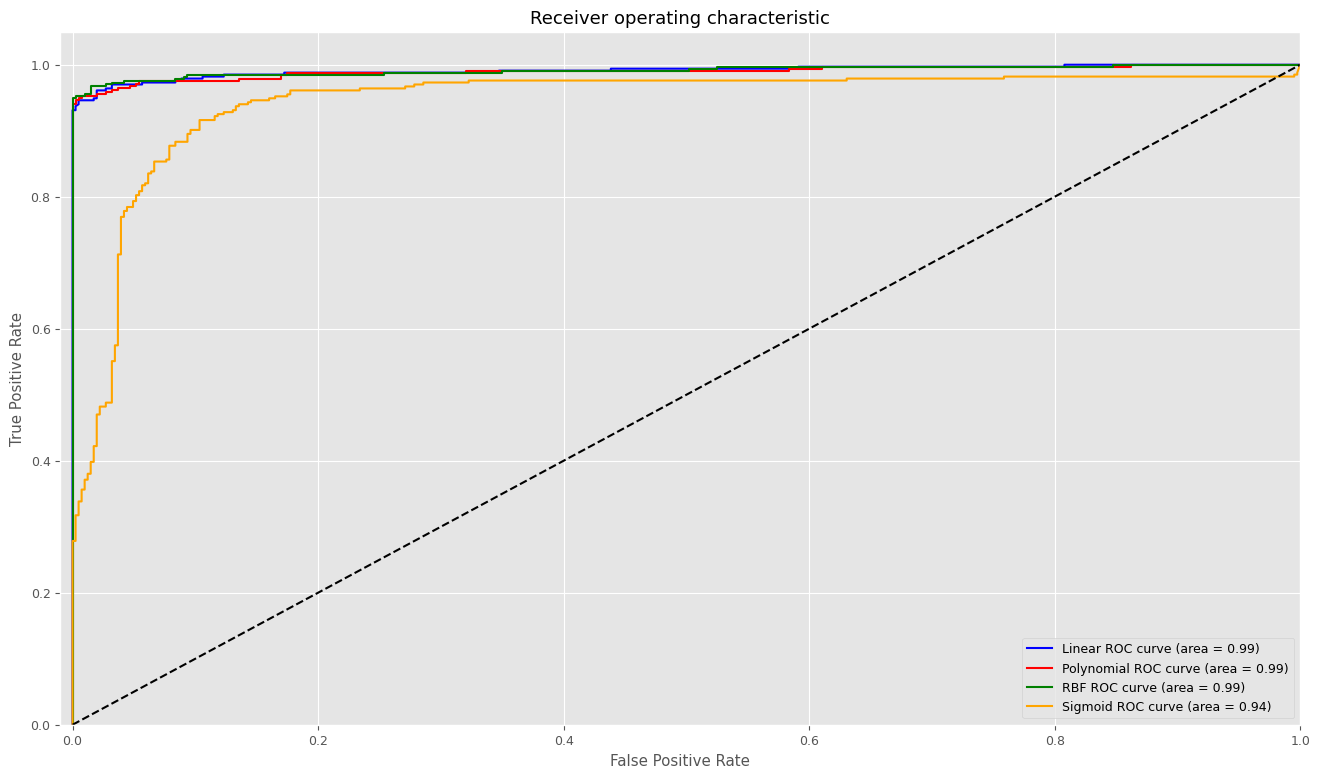
\includegraphics[width=0.75\textwidth]{img/svm/SVM_roc_pca.png}
    \caption{Curva ROC dei vari kernel SVM a confronto su dataset PCA}
    \label{fig:roc_SVM_PCA}
\end{figure}

Come per il modello precedente, anche sul \texttt{dataset\_pca\_std} non si hanno particolari
differenze tra i vari kernel esclusa la sigmoide. Si nota inoltre che dal
grafico \ref{fig:roc_SVM_PCA} non è possibili distinguere quale kernel sia
il migliore in quanto le curve ROC sono molto simili tra loro e l' AUC è la
stessa per più kernel, quindi la scelta è stata effettuata unicamente in base
ai risultati delle metriche principali. Dalle metriche si denota che il miglior
kernel è RBF, quindi SVM\_pca sarà definito dai seguenti parametri:
\begin{itemize}
    \item kernel: $RBF$
    \item $C$: $100$
    \item $\gamma$: $auto$
\end{itemize}

\newpage
\section{Gaussian Naive Bayes}
In questa sezione verranno brevemente descritti i
modelli candidati per \textbf{Gaussian Naive Bayes} (GNB). A differenza
degli altri algoritmi, l'unico iperparametro da stimare sarebbe la Prior che
dovrebbe essere specificata da esperti del dominio. Essendo che le nostre
competenze su tale dominio non ci permettono di determinare il valore corretto
abbiamo deciso di non specificare il suo valore.
Non specificando la Prior, la libreria sklearn le stimerà automaticamente 
dal dataset.

Con le suddette premesse sono stati definiti i due modelli:
\begin{itemize}
    \item GNB\_corr: modello allenato e valutato sul dataset \texttt{dataset\_corr}
    \item GNB\_pca: modello allenato e valutato sul dataset \texttt{dataset\_pca}
\end{itemize}

\section{Rete Neurale}
In questa sezione verrà presentata la \textbf{rete neurale}. Nello specifico, si
andranno a presentare i passaggi che sono stati effettuati per la realizzazione
dei due modelli, prestando particolare attenzione alla fase di definizione
della struttura delle reti neurali e alle fasi di addestramento della stesse.

Tutte le operazioni effettuate sono state realizzate utilizzando i dataset standardizzati
(\texttt{dataset\_corr\_std} e \texttt{dataset\_pca\_std}) presentati nella fase
di preparazione dei dati, in modo da rispettare il più possibile le assunzioni
delle reti neurali, anche se una feature non rispetta l'ipotesi di normalità.

In questa sezione verranno presentati i seguenti modelli:
\begin{itemize}
    \item NN\_corr: utilizza NN su \texttt{dataset\_corr\_std}
    \item NN\_pca: utilizza NN su \texttt{dataset\_pca\_std}
\end{itemize}

\subsection{Modello NN\_corr}
Per svolgere il compito di classificazione si è scelto di utilizzare una rete
neurale feedforward, la cui struttura, a meno del layer di input e di output, è
stata definita attraverso il processo di grid search insieme agli iperparamentri.
La grid search si è articolata attraverso una cross validation a $5$ fold sul training
set di \texttt{dataset\_corr\_std}.

Dai risultati ottenuti dalla fase di analisi e dal dominio del problema, si è
scelto di utilizzare una rete con una struttura di dimensioni ridotte, in modo
tale da ridurre i tempi di addestramento e ridurre la possibilità che la rete
neurale soffra di overfitting.

\subsubsection{Ottimizzazione degli iperparametri}
Come già accennato in precedenza, la ricerca degli iperparametri della rete neurale
è stata effettuata attraverso un processo di grid search. Questo processo ha
permesso di valutare le prestazioni della rete neurale al variare della funzione
di attivazione, del numero di layer nascosti e del numero di neuroni per ogni
layer nascosto.

Per le motivazioni espresse nella sezione precedente sulla dimensione della rete,
l'operazione di grid search è
stata effettuata prendendo in considerazione un numero di neuroni per layer
tra 5 e 10 mentre il numero di layer nascosti è stato valutato tra 1 e 2.

Per quanto riguarda la funzione di attivazione, sono state valutate le seguenti
funzioni di attivazione:
\begin{itemize}
    \item \textit{ReLU}
    \item \textit{Leaky ReLU}
    \item \textit{sigmoid}
\end{itemize}

\begin{figure}[!ht]
    \centering
    \begin{subfigure}[b]{0.3\textwidth}
        \centering
        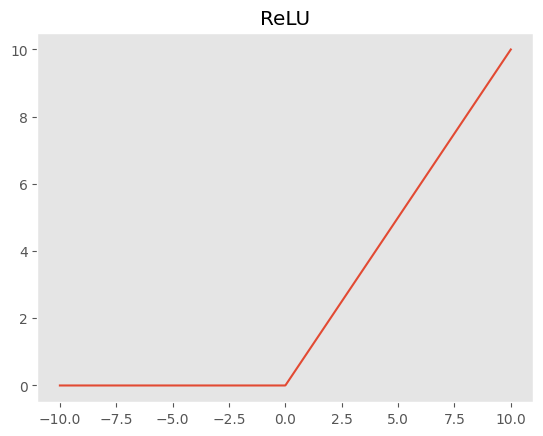
\includegraphics[width=\textwidth]{img/rete/relu.png}
        \caption{ReLU}
        \label{fig:relu}
    \end{subfigure}
    \hfill
    \begin{subfigure}[b]{0.3\textwidth}
        \centering
        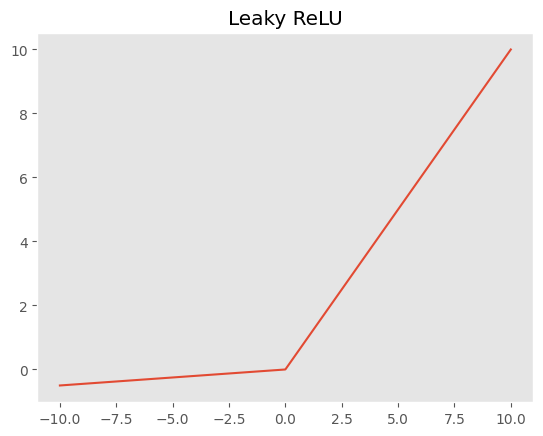
\includegraphics[width=\textwidth]{img/rete/leaky_relu.png}
        \caption{Leaky ReLU}
        \label{fig:leaky-relu}
    \end{subfigure}
    \hfill
    \begin{subfigure}[b]{0.3\textwidth}
        \centering
        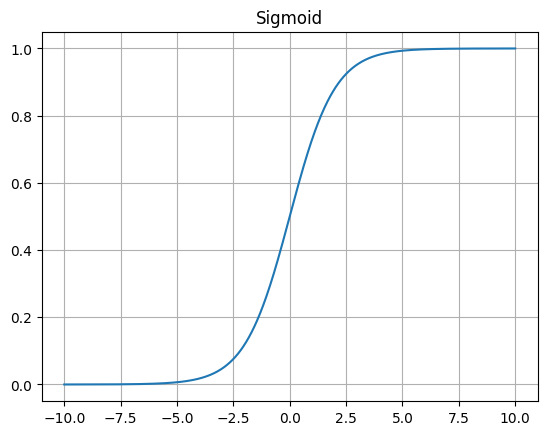
\includegraphics[width=\textwidth]{img/rete/sigmoid.png}
        \caption{Sigmoide}
        \label{fig:sigmoid}
    \end{subfigure}
    \caption{Funzioni di attivazione utilizzate nella fase di grid search}
    \label{fig:}
\end{figure}

Durante il processo di grid search, per ogni modello che è stato addestrato, sono
state raccolte delle informazioni relative all'accuratezza e al tempo di addestramento
richiesto. Quindi per ogni combinazione di parametri, sono stati calcolati gli
intervalli di confidenza al $90\%$ delle metriche e le rispettive medie.

Ottenuti i risultati, si è proceduto con l'analisi di questi, in modo tale da
definire la struttura della rete neurale. Per effettuare questa valutazione sono
state utilizzate le misure precedentemente citate.

La combinazione migliore è stata scelta attraverso i seguenti passaggi:
\begin{itemize}
    \item Calcolo della dimensione degli intervalli di confidenza, in modo tale
          da valutare la variabilità delle prestazioni della rete neurale.
          Questa operazione è stata effettuata sia per l'accuratezza, sia per il
          tempo di addestramento, calcolando la differenza tra il massimo e il
          minimo valore dell'intervallo di confidenza.
    \item Assegnazione di un punteggio di ranking per ogni metrica calcolata, in modo tale
          da valutare la posizione di ogni modello nella classifica.
    \item Calcolo del modello migliore attraverso la seguente formula considerando
          la posizione nella classifica di ogni modello per ogni metrica calcolata:
          \begin{center}
              \textit{RankModello = 2 * Rank accuracy + 2 * Rank tempo di addestramento + 1 * Rank dimensione intervallo di confidenza della accuracy + 1 * Rank dimensione intervallo di confidenza del tempo di addestramento}
          \end{center}
\end{itemize}

Nello specifico, per calcolare il punteggio di ranking della combinazione di parametri,
sono stati utilizzati i seguenti pesi: 2 per l'accuratezza
media, 2 per il tempo di addestramento medio e 1 per gli intervalli di
confidenza. Questi pesi sono stati scelti in modo tale da dare più importanza
all'accuratezza media e al tempo di addestramento medio, in quanto sono le due
misure che permettono di valutare le prestazioni della rete neurale, mentre gli
intervalli di confidenza sono stati utilizzati per valutare la variabilità delle
prestazioni.

Per verificare se il punteggio di ranking definito precedentemente è affidabile,
si è proceduto con il confronto dell'accuratezza media e del tempo medio tra la combinazione
migliore, la combinazione col tempo medio minore e la combinazione con l'accuratezza
media maggiore, ottenendo i risultati riportati in tabella \ref{tab:ris-grid-search}.
\begin{table}[ht]
    \centering
    \begin{tabular}{@{}lcc@{}}
        \toprule
        \rowcolor[HTML]{EFEFEF}
        \multicolumn{1}{c}{\cellcolor[HTML]{EFEFEF}\textbf{Combinazione di parametri}} & \textbf{Accuratezza} & \textbf{Tempo di addestramento} \\ \midrule
        Combinazione col tempo medio minore                                            & 98.31\%               & 1.84s                           \\
        Combinazione con l'accuracy media maggiore                                     & 99.05\%               & 17.74s                          \\
        Combinazione migliore rispetto al ranking pesato                               & 98.65\%               & 2.29s                           \\ \bottomrule
    \end{tabular}
    \caption{Risultati ottenuti dalla fase di grid search}
    \label{tab:ris-grid-search}
\end{table}

Dai valori riportati nella tabella \ref{tab:ris-grid-search} si può notare che
la combinazione di parametri  che è stata selezionata fornisce un compromesso tra
accuratezza e tempo di addestramento. Nello specifico, perdendo lo $0.4\%$ di
accuratezza media si è ottenuto un tempo di addestramento medio minore di circa $15$ secondi.

\subsubsection{Definizione della struttura del modello}

I risultati ottenuti dalla fase di grid search hanno permesso di definire la
struttura interna del modello. In particolare, il modello sarà composto da $1$
layer di input, $2$ layer nascosti e $1$ layer di output.

Dal momento che \texttt{dataset\_corr\_std} è composto da $5$ feature, questo ci ha permesso
di definire la struttura del layer di input per il modello NN\_corr, ovvero
$5$ neuroni di input, uno per ogni feature del dataset.

I layer nascosti sono composti nel seguente modo:
\begin{itemize}
    \item Il primo layer nascosto è composto da $10$ neuroni, in cui la funzione di
          attivazione è la funzione \textit{Leaky ReLU} \ref{fig:leaky-relu}.
    \item Il secondo layer nascosto è composto da $10$ neuroni, in cui la funzione
          di attivazione è la funzione \textit{Leaky ReLU} \ref{fig:leaky-relu}.
\end{itemize}

Per concludere la descrizione del modello, è necessario specificare come è composto
l'ultimo layer, ovvero quello di output. Vista la natura del problema di classificazione,
il layer di output è composto da un solo neurone, in cui la funzione di attivazione
è la funzione sigmoide \ref{fig:sigmoid}.

\begin{equation}
    \sigma(x) = \frac{1}{1 + e^{-x}}
\end{equation}

Questa scelta è dovuta al fatto che tale funzione restituisce un valore compreso
tra $0$ e $1$, il che permette di interpretare l'output della rete neurale come la
probabilità che l'input appartenga alla classe \textbf{positiva}.

La struttura della rete neurale è riassunta nella figura \ref{fig:strutturaReteNeurale}.

\begin{figure}[!ht]
    \centering
    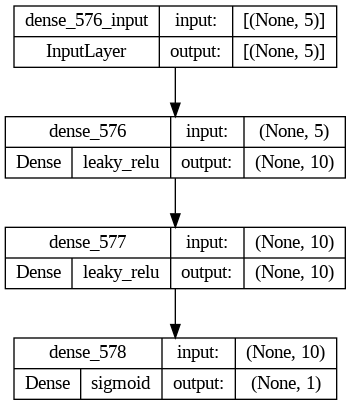
\includegraphics[width=0.3\textwidth]{img/rete/struttura_rete.png}
    \caption{Struttura della rete neurale}
    \label{fig:strutturaReteNeurale}
\end{figure}

\subsubsection{Altri iperparametri}
Oltre alla ricerca della struttura della rete neurale, la fase di grid search è
stata utilizzata per valutare l'algoritmo di ottimizzazione, il numero di epoche
e la dimensione del batch. Questi ultimi parametri saranno utili per le fasi di training
nel modello sopra descritto.

Per quanto riguarda l'algoritmo di ottimizzazione, il confronto è stato eseguito
tra \textit{Adam} e \textit{SGD}, mentre per il numero di epoche e la dimensione
del batch sono stati valutati rispettivamente i seguenti insiemi di valori: $100$, $300$ e $50$,
$100$, $300$.

I risultati ottenuti dalla fase di grid search hanno permesso di definire i valori
degli iperparametri che hanno permesso di ottenere i migliori risultati. In
particolare, l'algoritmo di ottimizzazione scelto è \textit{Adam}, mentre il
numero di epoche e la dimensione del batch sono stati impostati rispettivamente
a $100$ e $300$.

In questa fase è stato necessario definire la funzione di perdita. Si è scelta
la \textit{binary crossentropy} in quanto adatta a problemi di classificazione
binaria. La scelta di questa loss è dovuta alla natura del problema di
classificazione che si vuole risolvere.

\subsection{Modello NN\_pca}

Come per la definizione del modello NN\_corr, anche per questo modello sono stati
ottimizzati gli stessi iperparametri con le medesime metodologie, ma tutto applicato
su \texttt{dataset\_pca\_std}. Dal momento che il processo è analogo a quello
effettuato per il modello precedente, sia a livello di iperparametri, sia a livello
di valutazione delle combinazioni, allora in questa sezione verranno presentati
solo i risultati ottenuti.

Come fatto in precedenza, la combinazione migliore di parametri è stata confrontata
con la combinazione che ha ottenuto la migliore accuratezza media e la combinazione
che ha ottenuto il miglior tempo di addestramento medio. I risultati ottenuti sono
riportati in tabella \ref{tab:ris-grid-search-pca}.

\begin{table}[ht]
    \centering
    \begin{tabular}{@{}lcc@{}}
        \toprule
        \rowcolor[HTML]{EFEFEF}
        \multicolumn{1}{c}{\cellcolor[HTML]{EFEFEF}\textbf{Combinazione di parametri}} & \textbf{Accuratezza} & \textbf{Tempo di addestramento} \\ \midrule
        Combinazione col tempo medio minore                                            & 96.89\%              & 1.13s                           \\
        Combinazione con l'accuracy media maggiore                                     & 98.14\%              & 1.37s                          \\
        Combinazione migliore rispetto al ranking pesato                               & 98.07\%              & 1.29s                           \\ \bottomrule
    \end{tabular}
    \caption{Risultati ottenuti dalla fase di grid search}
    \label{tab:ris-grid-search-pca}
\end{table}

Anche in questo caso, come nel precedente, la combinazione selezionata 
rappresenta un compromesso tra l'accuratezza media e il tempo medio di 
addestramento. In particolare, aumentando di circa $0.16$ secondi il tempo di 
addestramento, l'accuratezza media aumenta di circa il $2\%$. Inoltre, la 
differenza tra la combinazione che offre la maggiore accuratezza media e la 
combinazione migliore secondo il ranking pesato è piuttosto ridotta ($0.07\%$).

I risultati ottenuti dalla fase di grid search hanno permesso di definire la
struttura della rete neurale. In particolare, la rete neurale è composta da $1$
layer di input, $2$ layer nascosti e $1$ layer di output.

Il layer di input è composto da $3$ neuroni, uno per ogni componente principale
ottenuta attraverso la PCA. Questo primo strato è stato definito in questo modo
in quanto il dataset ottenuto attraverso la PCA è composto da $3$ feature.

I layer nascosti sono composti nel seguente modo:
\begin{itemize}
    \item Il primo layer nascosto è composto da $5$ neuroni, in cui la funzione di
          attivazione è la funzione \textit{Leaky ReLU} \ref{fig:leaky-relu}.
    \item Il secondo layer nascosto è composto da $10$ neuroni, in cui la funzione
          di attivazione è la funzione \textit{Leaky ReLU} \ref{fig:leaky-relu}.
\end{itemize}

Il layer di output è lo stesso utilizzato per il modello NN\_pca, ovvero è composto
da un solo neurone in cui la funzione di attivazione è la funzione sigmoide \ref{fig:sigmoid}.

\begin{figure}[!ht]
    \centering
    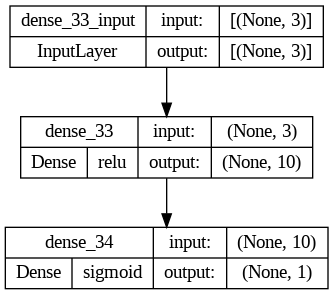
\includegraphics[width=0.3\textwidth]{img/rete/struttura_rete_pca.png}
    \caption{Struttura della rete neurale addestrata con PCA}
    \label{fig:strutturaReteNeuralePCA}
\end{figure}

Per quanto riguarda l'algoritmo di ottimizzazione, il confronto è stato eseguito
tra \textit{Adam} e \textit{SGD}, mentre per il numero di epoche e la dimensione
del batch sono stati valutati rispettivamente i seguenti insiemi di valori: $100$, $300$ e $50$,
$100$, $300$.

Per quanto riguarda gli iperparametri legati al training del modello, sono stati
rispettivamente scelti i seguenti valori:
\begin{itemize}
    \item Ottimizzatore: \textit{SGD}
    \item epoche: $100$
    \item batch size: $300$
\end{itemize}

Infine la loss scelta rimane sempre \textit{binary crossentropy}.